\chapter{团队协作} % Introduction chapter suppressed from the table of contents

客户:极限编程(eXtreme Programming)强调团队要共同拥有代码,这条看起来很容易理解,但又很难理解。

我们一起写程序当然是一起负责,道理很简单,但为什么会有这一条原则?背后有什么原因?然后这章节会探索作为编程员和管理员,怎么才才算做好这一点?

我:讲需求与开发已强调团队合作很重要,但没有探索针对软件开发团队心理问题,之前的英国煤矿“长壁”机械采煤案例证明不能单靠正式的组织架构和科学管理方式设计工作流程,来管理团队。因为实际的情况变化万千,必须依赖团队成员之间相互合作,才可以有效提高生产力和矿工的心态健康。\\

我:现在公司新人也很多,怎么识别谁是开发?\\
客户:很简单,不喜欢说话,不跟人家交流,每天沉迷在电脑前面那些人,肯定是开发人员。\\
我:一般人有这种概念,就是开发都是单独和富于创作性的,他们喜欢自己创作,不希望被打扰。员工专注做好工作,原本是好事,但如果做得过的时候,反而会产生负面影响。\\
客户:为什么?\\
我:因程序员越来越觉得程序是自己的作品,好像自己写了本书,在封面有自己的大名一样,但是软件和艺术作品不一样,如果有反对声音,觉得他作品不好,艺术家会认为是你不懂。但是软件程序不一样,它最后是在电脑运行,运行有错误就是有错误,所以导致程序员都会想尽办法证明自己的程序没错,问题不是出自自己。

一般人都会觉得自己比他人出众,如果做得好,觉得是自己棒;如果做错了,就是题目太难了,不是自己的问题。

为了平衡这个心理,一般人会想尽办法找理由说明问题不在自己。

程序员的心理(比矿工)更加高深莫测,这问题从60年代软件开发的萌芽期已经存在,不信可先看看以下故事:

\hypertarget{ux5404ux81eaux8d1fux8d23ux81eaux5df1ux5f00ux53d1ux7684ux6a21ux5757}{%
\subsection{各自负责自己开发的模块}\label{ux5404ux81eaux8d1fux8d23ux81eaux5df1ux5f00ux53d1ux7684ux6a21ux5757}}

60年代,当程序还需要操作人员用机器把程序打在一堆卡片(一行一张卡片),然后利用读卡器把程序输入电脑的时代,如果程序有误,编程员会说是输入员出错,或者说是卡片的顺序错了。\\
%\href{文件:cleanagile_f3.3.jpg}{200px}
%\href{文件:cleanagile_f3.4.jpg}{200px}

\includegraphics[width=10cm]{cleanagile_f33.jpg}\\
\includegraphics[width=10cm]{cleanagile_f34.jpg}\\

你可以想象,如果程序员有这种心态,对整个团队的质量和交付都不好。所以我们每个人要抛弃拥有自己程序的心态,不要认为这是个人的作品,而是属于大家的,他会更能接受错误,对软件的质量有好处。

在实际工作环境中,大部分的软件都是有一组人合作写的,很少能靠单一个人完成。

\hypertarget{ux56e2ux961fux5408ux4f5c}{%
\subsection{团队合作}\label{ux56e2ux961fux5408ux4f5c}}

当项目需要多人合作,各有所长和所短,也出于更好满足需求,自然会形成一个团队合作模式,各人互补。当这个团队形成以后,团队成员会互相依赖,不轻易换人。例如某个团队预计公司会有计划解散这个团队,队员就开始寻找新的工作机会。最后这个团队选择一起离开,入职另外一家公司。新公司的经理觉得过来这些人都挺靠谱的,软件交付质量不错,当他有一些比较重要不能延误的开发工作,都会交给团队的其中一位。但他有所不知,虽然他是交给其中一位小李,但实际上工作是由团队内部相互合作完成的,不是一人的工作。

从这个例子看到,一旦团队形成相互合作模式,它的作用要大于每个个人相加,也正因为如此,也正因为这个原因,团队会很慎重处理新成员的加入。假如有新人进来的时候会先告知新人,必须遵守团队的交付规则。例如后面加入了一位新人,他有3年开发经验的``老''程序员,觉得自己有经验,不需要遵循这一套规则,还是用自己的方式去开发,但越来越发现他的交付质量跟不上团队。最后有一次他交付了自认为是``良好''没有缺陷的程序给团队。为了避免再出事,他的程序被交给一位与他同时加入团队的实习生审查(这实习生加入后一直按团队规则交付,所以进步很快),他觉得很没有面子,最后他无法接受就辞职了。\\
这种情况不仅在软件开发团队存在,在合唱团或弦乐四重奏团也一样,非常依赖互相合作,所以在选择新成员方面非常谨慎,不要求个人英雄,更重要是要能跟其他人合作。

从以上例子看到,成功的团队是软件开发公司的宝贵资产,但管理者应该怎么去管理呢?要注意管理程序员这些知识工作者,不要用管理工人那种心态。比如下面这两个例子。\\

\hypertarget{ux6309ux65f6ux4e0aux4e0bux73ed}{%
\subsection{按时上下班}\label{ux6309ux65f6ux4e0aux4e0bux73ed}}

某大型项目中途换了部门经理,新加入的经理发现经常有程序员早上10点半才上班,他没有去问原因(其实有些程序员前一天晚上工作到凌晨两点钟),觉得这些情况直接影响团队管理,要立马改正,避免大家漠视公司规则偷懒,立马发通知要求大家要按公司规定时间上下班。\\
程序员立即集体反应:\\
完全按照经理的要求准时上班,也准时5点15分清理好桌面下班,并一起排队去打卡。但因为本来这些团队都默认按轮班制,有些早到、有些晚去对应电脑时间的限度(60年代机器没现在发达,写好程序打完一堆程序卡片后,都是要排队让电脑按序运行)。经理发了这个通知后,生产率立马降低一半,很多程序员白天没事干,等机器有空才可以工作,然后电脑也按公司的时间运行,到下班时间就立刻停机。\\
60年后的现代,也会看到同类故事在软件开发公司发生。\\

\hypertarget{ux4ec0ux4e48ux5bfcux81f4ux7cfbux7edfux5d29ux6e83}{%
\subsection{什么导致系统崩溃}\label{ux4ec0ux4e48ux5bfcux81f4ux7cfbux7edfux5d29ux6e83}}

%\href{文件:TC6stagesNioScreenshot_2022-10-27_192322.jpg}{400px}
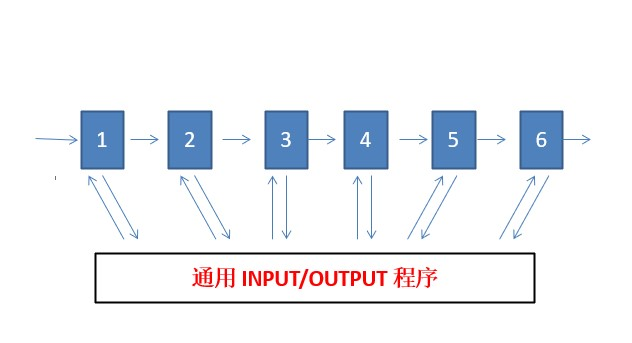
\includegraphics[width=10cm]{TC6stagesNioScreenshot_2022-10-27_192322.jpg}\\

有一个大型项目,希望把一个以前在老版本主机运行的应用软件系统更新到新硬件平台,总费时超过两年,团队平均人数在10位左右。这系统本来已经运作很成熟,所以整个开发最关键的部分就是更新硬件的接口部分,其他模块的开发相对简单。项目比较大,必须要分成6个阶段,其中有人负责这个重要的接口部分,其他人就负责原有模块的软件升级。过了一年半,一切的测试进展都很顺利,到了第5个阶段的验收测试就发现出问题了,整个机器就停下来了。距离交付只有不到2个月的时间,大家就赶紧去找问题,仔细查看所有第5阶段的相关代码和接口部分的代码,测试之后和原有的比较没发现任何问题。

没办法,就在加人手研究之前的第4部分,还是没有任何进展,时间也越来越紧了,大家很着急,又加了一些新的人来加入研究,因为开发时间比较长,有些之前阶段的人员都已经离开了。有一次,小张(他刚进入团队)与一位原本团队成员喝咖啡聊天,听到那位``老''员工回忆刚开始分工时,有一位特别厉害的程序员唐工,他非常不满意分工安排,他认为自己是团队里面最有经验最有能力的,他不满意接口部分的编程交给了李工负责。唐工一直闷闷不乐,一周之后才平静下来。

小李听完以后立马有了灵感,就问唐工当时负责哪个阶段?哪个模块?那个老员工说:“他负责第二个阶段的那些模块。”这个小李回去立马查看第2个阶段模块的代码,很快便有发现,程序一开始就在内存里面读一个变量,然后把整个程序从那个接口调到唐工写的模块运行。原来唐工因为不满安排,写他负责部分的程序时,绕过李工负责的接口模块,让自己的第二模块直接对接,不用本来的接口。因他编程很厉害,做完这个动作后还让原本的变量原封不动,大家很难看出来。但因为他改变内存里那些记录,外围那些机器,如磁带机,因内存记录错误,就被搞乱了,所以一直到第4阶段都没有异常,但到第五阶段的时候就引起整个系统崩溃。

从上面的例子看到,软件协作并不是一件简单的事,外人很难看出其中做了什么手脚。如果我们分工时,没有真正让每个成员满意,也没有注意某些成员的心理不平衡,可能会导致灾难性后果。

\hypertarget{ux6280ux672fux56e2ux961fux7684ux6301ux7eedux6027}{%
\subsection{技术团队的持续性}\label{ux6280ux672fux56e2ux961fux7684ux6301ux7eedux6027}}

保持团队持续性也很重要,因为成员会离开,当处理不当的时候,将会引起灾难。\\
例如公司小李很有魄力和经验,下面有两位实习生帮助他。但是为了这个程序,他长期离家到偏远的现场工作,想尽快回家,于是向经理申请:“咱公司小张在这块也有经验,如果可以让他过来学习这个怎么做,我就可以派去做其他项目。”

但碍于小张正在做另外一个项目,经理不想调走小张,因为又要找到另外一个人代替。所以为了满足小李的要求,经理给他多增配一位实习生,但这对小李一点帮助没有,增加实习生只是增加他的负担。所以小李就再去对经理申请说:``不行了,你还是快点找小张过来帮我吧。''

经理最后的解决办法是给小李增加了25%薪水,希望他留下来,但过了不到1周,小李辞职了。

经理最终没有其他选择,只能派小张接管这个项目。但因为他没有受过任何相关的培训,还是一团糟。过了几个月,这个项目出不了预期的效果,最后被取消了,对公司造成很大的损失。\\
从刚才的故事可以看到,一般经理以为薪水可以代替一切,其实不一样。对小李来说,加薪水就是希望他留下来,但是他就是不想留下来,所以这个加薪水反而变成他辞职的催化剂。从这个案例有两个经验教训:

\begin{itemize}
\tightlist
\item
  每个项目每个岗位都应该有备份,如果有任何一个岗位不能有人代替的话,后面的风险极大,必须立马处理。
\item
  我们对程序员不能用一般管工人的心态,不是用钱就可以解解决一切问题。\\
\end{itemize}

从以上的例子看到管理开发团队要注重成员的心理状态。这个道理其实对任何团队协作的工作都适用,但对于软件开发这种偏知识性行业则特别重要。因为每个开发人员都会觉得自己是高手,如果这块心理得不到平衡,他会用各种方式去平衡,甚至会对整个团队的表现产生负面影响。

客户:听完你这些开发团队的小故事,我作为管理者是否应该放手尽量少干预,让团队自主管理,类似庄子那种无为而治道家思想就好了吗?\\
我:不一定,如果你只是放手团队自我管理,没有任何要求,团队很容易就会没有动力,后果也很严重,可以看看以下实例。\\

\framebox{%
\begin{minipage}[t]{0.97\columnwidth}\raggedright
某回国技术总监的经历\\
刚回国不久,还帮日本公司带领小团队做开发,这时有个朋友找我,说他的团队经常被客户投诉,请我帮忙看看。我就到这家公司,因为大老板以前是学校的老师,没有投入足够精力管理公司。本来这公司的团队管理模式很自由,每个人和团队都非常独立,大家互相不干扰。团队一直帮客户做开发与维护,客户觉得这个合作习惯了,也不想转变或换人,导致开发人员的效率和质量都不高。因为管理层也比较放松,开发人员也没什么压力,只要服务到客户不投诉就行。也没有任何规范和指标。我观察了一段时间,帮他们做一些辅导咨询,后面老板比较信任我的能力,于是邀请我来管理团队,我答应了。\\

我发现加入以后,管理他们更难了。比如我希望他们按我的要求有计划地加强管理,他们并不听。有时我觉得有些员工能力不够,需要调走,但他和客户关系好,客户立刻和我说,不能动这个人,否则我就不再继续签合同。这些开发人员已经是“老油条”,知道用什么手段保护自己,尽量不发生任何改变。我没有办法影响他们的话,团队就无法进步,于是建议大老板说,我们废除以前根据主管打分决定员工薪水的方式,而是做成“奖金池”,用客观的方式来判断员工的贡献,而不是靠主管的主观判断。奖金是按开发出来的功能点数量,开发越多奖金越高,功能点规模是由独立的QA依据开发的软件客观算出。开始时,效果挺好的,因为有客观数据的衡量。但是几年后,他们熟悉了之后,就开始玩花招。听你说团队持续改进的方式,我觉得可以尝试,让团队有下一波良性发展,提高他们的开发和创新能力。
\strut
\end{minipage}}

\framebox{%
\begin{minipage}[t]{0.97\columnwidth}\raggedright
作为管理者不是插手、替代团队做他们的工作,例如编程、计划等,但需要设定高的提升目标,帮助他们自己提升,才能持续保持公司和团队的竞争力,不然这很容易被自然淘汰。在这个过程中,也要注意开发人员的心态。激励不能单靠奖金,尽量要让他们形成团队,相互合作,对公司、个人都有好处。当团队成员能相互合作后,便可以帮助公司做好项目,满足客户需求。我看到很多团队成员在项目中间会被调走,这是常常影响到团队质量(与生产率)的主因。\\
客户:没办法,客户是上帝。比如他们有紧急维修要做,而只有一些有经验的开发能解决,就必须要占用他们时间,否则客户不满意。\\
我:但这种临时抽调的做法,会影响到他们正在做那些项目,也会引起客户不满。\\
客户:你有什么好建议?\\
我:我认为可以考虑下面敏捷大师Robert Martin的建议,他鼓励尽力保持团队不变,发挥团队相互合作关系的作用。\\
\strut
\end{minipage}}

\framebox{%
\begin{minipage}[t]{0.97\columnwidth}\raggedright
如何保持团队稳定\\
因为要让团队成员相互合作,变成有效的互补团队不容易,团队是公司的宝贵资产。所以当项目结束后,不应该解散团队,而是要分派新的项目,让团队可以继续合作。但有时候,项目的规模大小不一定能与团队匹配,可以考虑以下建议:\\
假如某团队的生产力是50个单位,就可以安排以下3个项目来让这团队负责,比如A项目需要15单位,B项目需要15单位,C项目需要20单位。如果某些项目后面突然间需要紧急加快速度,也可以很容易策划、改变分配的比例,这样会比平常增减人员简单很多。因为软件开发特别需要团队之间沟通,如果某项目需要加快速度,通常增加人手是没用的,原因是团队成员会花更多精力让新加入的成员融入。本来团队要教他们,在这种后面增加人员的情况,收益还不如在过渡培训的投入。有时候项目延误不是团队能力的问题,而是因为有紧急需要导致某些开发人员被调走,留下来的开发人员要兼顾老项目其他项目,同时要服务两三位项目经理,导致无法专注做好编码工作。所以太多骚扰会影响总体效率、生产率和质量。\\

\strut
\end{minipage}}

\framebox{%
\begin{minipage}[t]{0.97\columnwidth}\raggedright
应怎么安排呢?\\
要避免这种临时的抽调。但确实有些客户的紧急问题,只有某些开发人员熟悉,其他人不懂。\\
项目不应该有任何事情只有单一人懂,缺乏备份,要避免临时抽调,就必须策划好开发过程,团队不仅要做好产品开发跟交付,也需要把知识传递给软件维护团队,到后面出现事故时,就可以让维护团队处理,不打扰本来的开发团队,开发专注开发,维护专注维护。就可以避免这类对公司不利的抽调发生。 
\strut
\end{minipage}}

\hypertarget{ux9644ux4ef6}{%
\section{附件}\label{ux9644ux4ef6}}

\hypertarget{ux5e73ux8861ux5fc3ux6001-cognitive-dissonance}{%
\subsection{平衡心态 (Cognitive
Dissonance)}\label{ux5e73ux8861ux5fc3ux6001-cognitive-dissonance}}

\begin{itemize}
\tightlist
\item
  探索当行为和心理有冲突时,人们如何对应。
\item
  被安排做一些很沉闷的任务(例如扭螺丝钉)。
\item
  试验者会收到1美元或20美元,要他告诉下一个人这个任务很有趣,很有意义。
\item
  试验完成后,再问实验者对任务真正的感觉。
\end{itemize}

1957年实验,要求有些学生(被实验者)做一些很无聊的工作,比如反复钻螺丝、包装,后面给他1美元或者20美元。要他告诉下一位,刚才那个工作很有趣、很值得。实验后再问他们这个任务是否有趣?发现给1美元的人,大部分会觉得工作有趣。而给20美元的反而不同意觉得工作无聊。

原因:当你给他1美元的话,金额很小,他心里觉得不是被贿赂,所以会相信他自己说过的话。而当给了20美元,他觉得自己是收了那个钱才这样回答,否则肯定不会这么回答,所以心理上就会抗拒,不同意这个工作有趣。

分析实验结果:人会尽量说服自己``我做的是对的'',来取得心理平衡,所以即使他确实做的事很无聊,因为他跟人家说了这个事很有意义,他会尽量先说服自己,觉得这个是有意义,使自己心理平衡(收了1美元场景)。但反过来,当因为这件事收到20美金,他觉得这个说法不是自愿的,只是因为收了钱。反而就不需要动力去平衡自己的心态。\\

\hypertarget{ux9644ux4ef6}{%
\section{参考 References}\label{ux9644ux4ef6}}

1. Weinberg, Gerald. ''The Psychology of Computer Programming.''\\
2. Martin, Robert. ''The Clean Coder.''(2011)\\




